\section{Results}
\label{sec:results}

\todo{Add more results (matter of running more experiments, mostly)}

\subsection{Multi-model Translations}
Figure~\ref{fig:accuracy_multi_model_wikis} shows the accuracy of the multi-model translations, both for models trained on 100 and 400 dimensions. We used the same training set of translations to train the matrix on, and both language models are trained on respectively the Dutch and English Wikipedia.

An interesting observation is that the accuracy at all levels (top 1, top 5 and top 10) starts off lower for models trained at 400 dimensions. However, at the biggest training set, each level is better than the corresponding level at 100 dimensions. This suggests a form of overfitting; the translation matrix might be overfitted on the translation samples.

\todo{There's also a dip towards the end. Check if that's still there if we run it with differently split test/training data sets.}

\begin{figure}[ht!]
  \centering 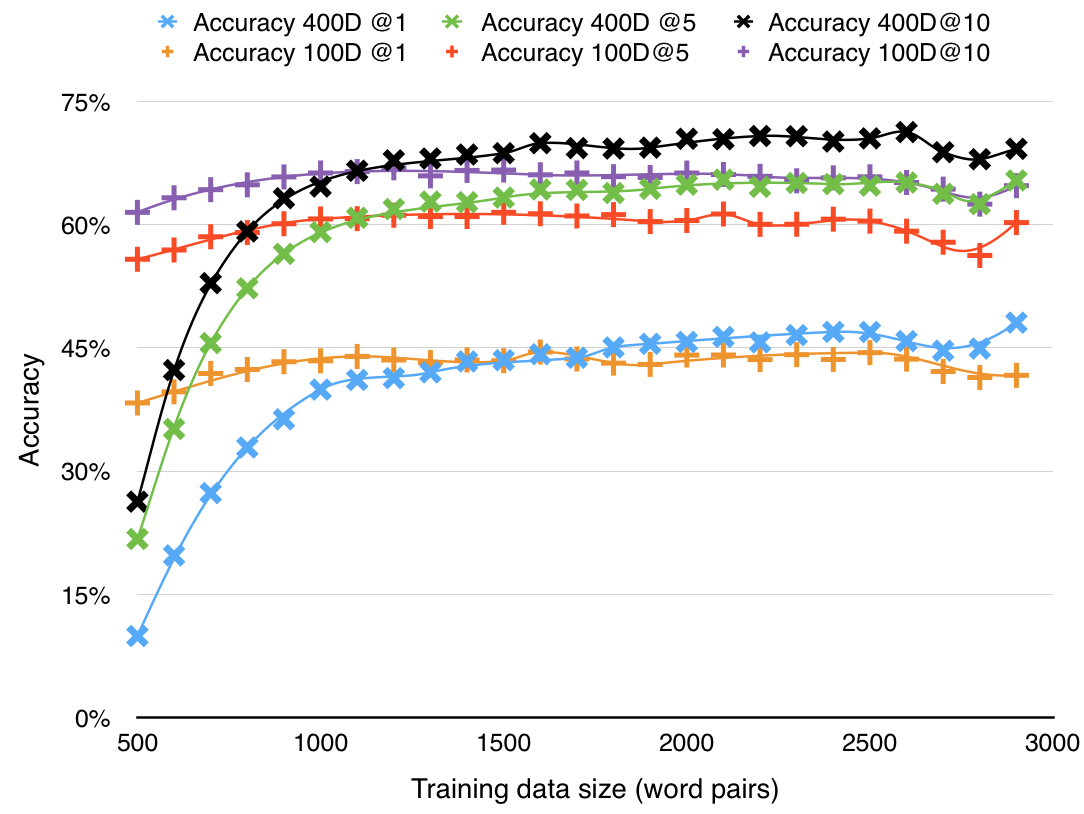
\includegraphics[width=\linewidth]{images/accuracy_multi_model_wikis}
  \caption{Accuracy for multi-model translations, trained on Dutch and English wiki. 'x' marks denote dimensionality 400, '+' marks dimensionalty 100.}
  \label{fig:accuracy_multi_model_wikis}
\end{figure}

\subsection{Single-model Translations}
In this section, we use two models: both are trained on the text of the English Wikipedia and the Dutch Wikipedia combined. Since the Dutch Wikipedia is much smaller than its English counterpart (by a factor of 8, see table~\ref{table:datasets}), we ran it eight times over the Dutch text. This artificially increases the weight given to Dutch text, so both are equally well represented.

The only difference between the two models is the number of dimensions: one is trained at 100, and the other at 400 dimensions.

\subsubsection{Using Relations}
To test the method described in section~\ref{sec:single-model-no-matrix}, we randomly select 100 translations from our testset of correct translations. For each of these translations, we then select 500 different translations to test against. This process is done both for a model trained at 100 dimensions, and one trained at 400 dimensions, and both for Dutch to English and vice versa.

Table~\ref{table:results_single_model_no_matrix} shows the results of these experiments.

\todo{Finish running tests...}
\begin{table}[ht!]
	\centering
	\label{table:results_single_model_no_matrix}
	\begin{tabular}{|l|l|r|r|r|r|r|r|}
	\hline
	\multirow{2}{*}{Direction} 	& \multirow{2}{*}{Func}	& \multicolumn{3}{c|}{100 dim}  		& \multicolumn{3}{c|}{400 dim} 	 \\ \cline{3-8} 
                  				&	 					& @1 		& @5 		& @10 	 		& @1 		& @5 		& @10 	 \\ \hline
    \multirow{2}{*}{NL$\to$EN}	& Avg					& 4.29\%	& 8.71\%	& 11.4\%		& 1.91\%	& 4.89\%	& 6.96\% \\ \cline{2-8} 
    							& Max					& 14.6\%	& 23.4\%	& 28.4\%		& 8.60\%	& 15.8\%	& 21.2\% \\ \cline{2-8} 
    							& Min					& 0.00\%	& 0.00\%	& 0.00\%		& 0.00\%	& 0.00\%	& 0.00\% \\ \cline{2-8} 
    							& Std					& 3.50\%	& 6.10\%	& 7.51\%		& 1.97\%	& 4.11\%	& 5.42\% \\ \hline
    \multirow{2}{*}{EN$\to$NL}	& Avg					& 3.92\%	& 8.28\%	& 10.9\%		& a\%		& b\%		& c\% 	\\ \cline{2-8} 
    							& Max					& 12.4\%	& 23.8\%	& 28.6\%		& a\%		& b\%		& c\% 	\\ \cline{2-8} 
    							& Min					& 0.00\%	& 0.00\%	& 0.00\%		& a\%		& b\%		& c\% 	\\ \cline{2-8} 
    							& Std					& 3.24\%	& 6.15\%	& 7.60\%		& a\%		& b\%		& c\% 	\\ \hline
	\end{tabular}
	\caption{Translation accuracy, using a single model without translation matrix and 400 dimensions.}
\end{table}







\subsubsection{Using Translation Matrix}
\todo{repeat experiment from multi model section, but use bothwiki 100 and bothwiki 400 as language models}
